\documentclass{article}
\usepackage{graphicx}
\usepackage[margin=1.5cm]{geometry}
\usepackage{amsmath}

\begin{document}
\twocolumn

\title{Friday Warm Up: Unit 5, Electromagnetism and Optics}
\author{Prof. Jordan C. Hanson}

\maketitle

\section{Memory Bank}

\begin{itemize}
\item \textbf{Optics:} Snell's Law states that, for an interface between two media with \textit{indices of refraction} $n_1$ and $n_2$, light leaves one medium with an angle $\theta_1$ and enters the second medium with an angle $\theta_2$ as follows:
\begin{equation}
n_1 \sin\theta_1 = n_2\sin\theta_2
\end{equation}
\noindent The two angles are defined with respect to vertical.
\item \textbf{Optics:} Fresnel's equations give the fraction of power (in light) that is reflected ($R$) or transmitted ($T$) by an interface between media with indices of refraction $n_1$ and $n_2$:
\begin{equation}
R = \left| \frac{n_1 - n_2}{n_1 + n_2} \right|^2 \label{eq:2}
\end{equation}
\noindent Note that, to conserve power, $T = 1 - R$.
\item \textbf{Thin lens equations}.  Let an object be a distance $d_{\rm o}$ from the center of a thin lens.  If the lens produces a real image at a distance $d_{\rm i}$ from the center of the lens on the opposite side from the object, $d_{\rm o}$ and $d_{\rm i}$ are related by the \textit{focal length} $f$:
\begin{equation}
\frac{1}{d_{\rm o}}+\frac{1}{d_{\rm i}} = \frac{1}{f}
\end{equation}
If the object has a characteristic size $h_{\rm o}$ and the image has a characteristic size $h_{\rm i}$, the \textit{magnification}, $m$, is
\begin{equation}
m = \frac{h_{\rm i}}{h_{\rm o}} = -\frac{d_{\rm i}}{d_{\rm o}}
\end{equation}
\item \textbf{Total internal reflection} occurs when light no longer refracts out of a material.  This occurs when the angle of incidence is greater than or equal to
\begin{equation}
\theta_{\rm C} = \sin^{-1}(n_2/n_1)
\end{equation}
\end{itemize}

\section{Fiber Optics, Snell's Law, and \\ Total Internal Reflection}

\begin{enumerate}
\item A light ray entering an optical fiber surrounded by air is first refracted and then reflected as shown in Fig. \ref{fig:1}. Show that if the fiber has $n_2 = 1.5$, with air having $n_1 = 1.0$, any incident ray will be totally internally reflected. \textit{Hint: pick a reasonable number for $\theta_1$, and work out $\theta_2$ and $\theta_3$.} \\ \vspace{3cm}
\end{enumerate}

\section{Lens Optics}

\begin{enumerate}
\item A certain slide projector has a 100 mm focal length lens. (a) How far away is the screen, if a slide is placed 103 mm from the lens and produces a sharp image? (b) If the slide is 24.0 by 36.0 mm, what are the dimensions of the image? \\ \vspace{4cm}
\item A dentist examines a patient using a 15.0 cm focal length eyepiece held 13.5 cm from their tooth.  (a) Where is the image? (b) What is its magnification? (c) How big is the image of a 10.00 mm diameter tooth?
\end{enumerate}

\begin{figure}
\centering
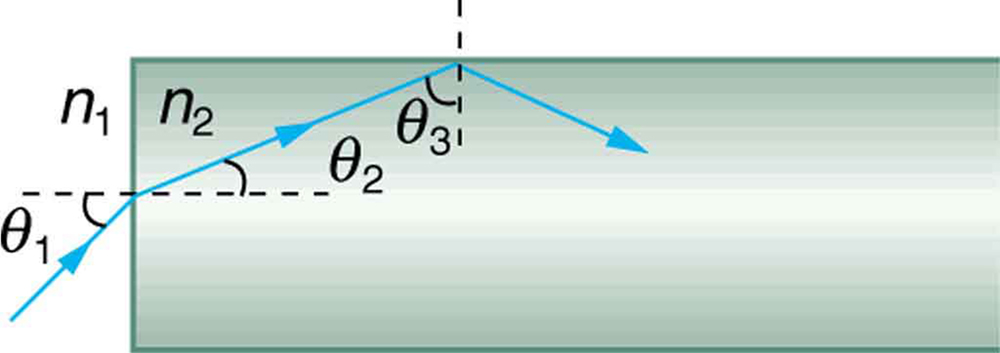
\includegraphics[width=0.48\textwidth]{figures/fibre.jpg}
\caption{\label{fig:1} A light ray enters a fiber optic cable.}
\end{figure}

\end{document}
